
%%%%%%%%%%%%%%%%%%%%%%%%%%%%%%%%%%%%%%%%%%%%%%%%%%%%%%%%%%%%%%%%%%%%%
%% This is a (brief) model paper using the achemso class
%% The document class accepts keyval options, which should include
%% the target journal and optionally the manuscript type.
%%%%%%%%%%%%%%%%%%%%%%%%%%%%%%%%%%%%%%%%%%%%%%%%%%%%%%%%%%%%%%%%%%%%%
\documentclass[journal=ancham,manuscript=article]{achemso}

%%%%%%%%%%%%%%%%%%%%%%%%%%%%%%%%%%%%%%%%%%%%%%%%%%%%%%%%%%%%%%%%%%%%%
%% Place any additional packages needed here.  Only include packages
%% which are essential, to avoid problems later.
%%%%%%%%%%%%%%%%%%%%%%%%%%%%%%%%%%%%%%%%%%%%%%%%%%%%%%%%%%%%%%%%%%%%%
\usepackage{chemformula} % Formula subscripts using \ch{}
\usepackage{achemso}
\usepackage[T1]{fontenc} % Use modern font encodings
\usepackage{amsmath}
\usepackage{subfigure}
\usepackage{amsfonts}
\usepackage{multirow}

%%%%%%%%%%%%%%%%%%%%%%%%%%%%%%%%%%%%%%%%%%%%%%%%%%%%%%%%%%%%%%%%%%%%%
%% If issues arise when submitting your manuscript, you may want to
%% un-comment the next line.  This provides information on the
%% version of every file you have used.
%%%%%%%%%%%%%%%%%%%%%%%%%%%%%%%%%%%%%%%%%%%%%%%%%%%%%%%%%%%%%%%%%%%%%
%%\listfiles

%%%%%%%%%%%%%%%%%%%%%%%%%%%%%%%%%%%%%%%%%%%%%%%%%%%%%%%%%%%%%%%%%%%%%
%% Place any additional macros here.  Please use \newcommand* where
%% possible, and avoid layout-changing macros (which are not used
%% when typesetting).
%%%%%%%%%%%%%%%%%%%%%%%%%%%%%%%%%%%%%%%%%%%%%%%%%%%%%%%%%%%%%%%%%%%%%
\newcommand*\mycommand[1]{\texttt{\emph{#1}}}

%%%%%%%%%%%%%%%%%%%%%%%%%%%%%%%%%%%%%%%%%%%%%%%%%%%%%%%%%%%%%%%%%%%%%
%% Meta-data block
%% ---------------
%% Each author should be given as a separate \author command.
%%
%% Corresponding authors should have an e-mail given after the author
%% name as an \email command. Phone and fax numbers can be given
%% using \phone and \fax, respectively; this information is optional.
%%
%% The affiliation of authors is given after the authors; each
%% \affiliation command applies to all preceding authors not already
%% assigned an affiliation.
%%
%% The affiliation takes an option argument for the short name.  This
%% will typically be something like "University of Somewhere".
%%
%% The \altaffiliation macro should be used for new address, etc.
%% On the other hand, \alsoaffiliation is used on a per author basis
%% when authors are associated with multiple institutions.
%%%%%%%%%%%%%%%%%%%%%%%%%%%%%%%%%%%%%%%%%%%%%%%%%%%%%%%%%%%%%%%%%%%%%
\author{Valeria Fonseca Diaz}
\email{valeria.fonsecadiaz@kuleuven.be}
\author{Bart De Ketelaere}
\email{bart.deketelaere@kuleuven.be}
\author{Ben Aernouts}
\email{ben.aernouts@kuleuven.com}
\altaffiliation{Biosystems, Division of Animal and Human Health Engineering, Campus Geel, Kleinhoefstraat 4, 2440 Geel, Belgium}
\author{Wouter Saeys}
\email{wouter.saeys@kuleuven.be}
\affiliation[KU Leuven]
{KU Leuven, Mechatronics, Biostatistics and Sensors (MeBioS), Kasteelpark
Arenberg 30, 3001 Leuven, Belgium}
%%%%%%%%%%%%%%%%%%%%%%%%%%%%%%%%%%%%%%%%%%%%%%%%%%%%%%%%%%%%%%%%%%%%%
%% The document title should be given as usual. Some journals require
%% a running title from the author: this should be supplied as an
%% optional argument to \title.
%%%%%%%%%%%%%%%%%%%%%%%%%%%%%%%%%%%%%%%%%%%%%%%%%%%%%%%%%%%%%%%%%%%%%
\title[An \textsf{achemso} demo]
  {Cost-efficient unsupervised sample selection for multivariate calibration}

%%%%%%%%%%%%%%%%%%%%%%%%%%%%%%%%%%%%%%%%%%%%%%%%%%%%%%%%%%%%%%%%%%%%%
%% Some journals require a list of abbreviations or keywords to be
%% supplied. These should be set up here, and will be printed after
%% the title and author information, if needed.
%%%%%%%%%%%%%%%%%%%%%%%%%%%%%%%%%%%%%%%%%%%%%%%%%%%%%%%%%%%%%%%%%%%%%
%\abbreviations{IR,NMR,UV}
\keywords{sample selection, multivariate calibration, NIR, PLS}

%%%%%%%%%%%%%%%%%%%%%%%%%%%%%%%%%%%%%%%%%%%%%%%%%%%%%%%%%%%%%%%%%%%%%
%% The manuscript does not need to include \maketitle, which is
%% executed automatically.
%%%%%%%%%%%%%%%%%%%%%%%%%%%%%%%%%%%%%%%%%%%%%%%%%%%%%%%%%%%%%%%%%%%%%

% -----------------------------------------------------
% -------------------BEGIN DOCUMENT ------------
% -----------------------------------------------------

\begin{document}


% -----------------------------------------------------
% ------------------- abstract  ------------
% -----------------------------------------------------
\begin{abstract}
Indirect quantification of chemical composition through spectral measurements requires the establishment of multivariate calibration models. The reference analyses on the calibration samples typically form a major cost factor in the establishment of these multivariate models. Therefore, the aim of this study was to select the most informative calibration samples in an unsupervised way based on the spectral measurements. To this end, guidelines to address this challenge in PLSR model building have been developed. The recommendations include calculating a sample size that surpasses the model complexity by a factor of 12, performing the selection in the PCA score space spanned by a sufficiently large number of principal components and using methods such as Kennard-Stone, Puchwein, Clustering or D-optimal designs.

\end{abstract}%

% -----------------------------------------------------
% ------------------- introduction  ------------
% -----------------------------------------------------

\section{Introduction}\label{introduction}

Combination of spectroscopic measurements with multivariate calibration models has become the primary analytical tool to indirectly measure the chemical composition of products making processes such as those of quality control more cost-efficient. However, the practitioner still faces many challenges when building and maintaining these models. One main challenge involves the selection of the calibration samples for which reference analyses have to be performed. To provide guidance related to this, an exhaustive evaluation of the challenge of unsupervised sample selection to build successful calibration models has been investigated in this study. Within the range of applications of multivariate calibration, the stated problem is particularly relevant for indirect inspection of collected or observed samples using near-infrared (NIR) spectroscopy. This characteristic of the samples is common in applications such as biomedical, environmental, mining, recycling and agrofood, the latter being one of the most relevant industries with increasing research in NIR applications \cite{Au2020,Diaz-Olivares2020, Saeys2005, Bobelyn2010}.

As spectral measurements are easy and cheap to collect, a vast quantity of units can be submitted to these measurements with low effort. On the contrary, collecting the reference analyses is a task that requires substantial effort, high costs and possibly high waste. The challenge of unsupervised sample selection relates to determining the best methodology or strategy to select the samples that would be worthy of reference analyses (chemical composition values), based on spectral measurements to build calibration models.
This has been the motivation to pay attention to the optimization of model building costs while gaining model building effectiveness. Historically, this has been rephrased as the optimal spanning of variability with a minimum number of samples \cite{Naes1990, Saeys2019,Kennard1969}.

Because of the importance of this problem, optimal sample sizes and suitable strategies to select these samples have been active research domains for many years \cite{Ferre1996,Au2020, Liu2019}. Through the last decades, many methods have been proposed for sample selection within a finite set of units. Some of these have become widely accepted for their intuitively accurate approach and good performance \cite{Shetty2012a, Nawar2018, He2015}. The two most popular methods in the context of NIR spectroscopy and multivariate calibration are the Kennard-Stone\cite{Kennard1969} and  Puchwein\cite{Puchwein1988} algorithms. As a strategy for sample selection, clustering techniques are widely accepted in order to account for multiple sources of variability\cite{Naes1990}, particularly when groups of samples exist in batches of collected products\cite{Bobelyn2010}. These popular algorithms have the common feature of relying on distance between the samples. Less popular in NIR applications but highly effective in product design are the D-optimal experimental designs, which translate the concept of variability from distance between samples to the variance of the coefficients of an assumed model \cite{Goos2011}. Yet, no clear understanding exists about which of all these methods are more suitable for NIR applications with multivariate calibration and no exhaustive evaluation of them has been disseminated. The most recent study found related to this problem used a selection method similar to the Puchwein algorithm and random selection to build models for the prediction of available nitrogen and total formylated phloroglucinol compounds in Eucalyptus leaves\cite{Au2020}. In the mentioned work, some guidelines were provided for the current problem, such as starting with a low number of samples and analyzing the crossvalidation error in order to decide whether more samples are needed to better train the calibration model. In addition, it was found that 200 samples accounted for a suitable sample size threshold in the prediction of available nitrogen ($N_{A}$)\cite{Au2020}. Although this sample size was suggested, no deeper analysis on the generality of it was provided. Another recent study related to the study on the sample size suggested a size threshold of 100 samples based on the evidence found with calibration models for grain, diary, petfood and compound food products \cite{Schoot2020}. In this latter study, the focus was mainly on the effect of the sample size for the effectiveness of preprocessing methods. Therefore, no profound analysis on the generalization of this sample size threshold was given.

Multivariate calibration is a concept that in principle can involve any type of statistical model for regression or classification \cite{Saeys2019}. The effectiveness of the type of bilinear models that are widely used for NIR applications has been reported by many researchers. Unless the spectral values have a strong nonlinear relationship with chemical reference values, bilinear models for regression tasks such as partial least squares regression (PLSR) or principal component regression (PCR) remain the workhorse model architectures\cite{FonsecaDiaz2020}. Most of the work that can be found addressing the current problem of interest provides answers about the minimum required sample size using PLSR models \cite{Naes1990, Au2020, Shetty2012a, Rodionova2008}. However, the diversity in the answers may confuse researchers rather than provide clear guidance. 

Therefore, the aim of this study was to provide a structured approach for the selection of the most informative calibration samples by understanding the properties of PLSR models. The general framework of statistical learning theory proposed by Vapnik provides specific guidelines for the sample size needed depending on the model architecture to be used\cite{Vapnik2019, Vapnik2000}. In order to apply these rules to multivariate calibration of spectroscopic sensors, PLSR has to be positioned within the framework explained by Vapnik. In a similar way, to understand the required features to take into account for a successful PLSR model, it is essential to seek for the elements of the PLSR architecture that can be controlled through unsupervised selection. In the remainder of this article, these aspects will be described and explained for the state-of-the-art methods for unsupervised selection of calibration samples.

A general framework and one specific for PLSR are presented in order to provide a context of analysis for finding the best strategy for unsupervised sample selection. The work is organized as follows: First, a description of the general and specific frameworks is presented as a basis to define the research questions of the current work. Next, the experimental work and results are presented along with the discussion of the aspects that lead to a more successful unsupervised sample selection to build calibration models. This culminates in a schematic guideline for efficiently selecting calibration samples. Finally, conclusions are drawn and suggestions for future research is presented.

% -----------------------------------------------------
% ------------------- frameworks  ------------
% -----------------------------------------------------

\section{Frameworks for analyzing properties of PLSR}

\subsection{Statistical learning theory as a general framework}

Statistical learning theory, as proposed by Vapnik\cite{Vapnik2019,Vapnik2000,Chapelle2002}, provides a general framework for analyzing the properties of PLSR. While PLSR has been presented as a particular case of the derived continuum regression \cite{Stone1990}, no reports were found on its positioning within statistical learning theory. From the perspective of Vapnik, in the general regression task, the response variable is assumed to be a linear combination of basis functions plus an error variable. With that model architecture and using a quadratic loss, the objective to estimate the model is to minimize the squared error \cite{Chapelle2002}. More concretely, let $y \in \mathbb{R}$ be the random variable representing the chemical constituent of interest and  $\mathbf{x} \in \mathbb{R}^{p}$ the predictor vector of spectral measurements. The regression model is defined as $y = f(\mathbf{x}, \boldsymbol{\beta}) + \epsilon$.  The general least squares regression problem can be established as \cite{Chapelle2002}:

\begin{equation}
    \min E \left[ (y-f(\mathbf{x}, \boldsymbol{\beta}))^2\right]; \quad f(\mathbf{x}, \boldsymbol{\beta}) = \sum_{k=1}^{\infty} \beta_k \phi_{k}(\mathbf{x})
    \label{eq_general_regression_problem}
\end{equation}

where $\{\phi_{i}(\mathbf{x})\}$ constitutes a basis of $L_2$ for which its elements can be ordered by some criterion. In the context of statistical learning theory, $E \left[ (y-f(\mathbf{x}, \boldsymbol{\beta}))^2\right]$ is called the \emph{expected risk}, which in practice is replaced by the designated \emph{empirical risk} in the presence of a set of $n$ observations to estimate function $f$ \cite{Vapnik2000}. This empirical risk is calculated as the sum of squared errors. The important feature of this optimization task is to ensure a small \emph{expected risk} by minimizing the \emph{empirical risk} only over a limited number of basis functions $\{\phi_{k}(\mathbf{x})\}_{k=1}^d$. Therefore, the regression problem becomes:

\begin{equation}
    \min \frac{1}{n} \sum_{i=1}^n (y_i-f_d(\mathbf{x}_i, \boldsymbol{\beta}))^2; \quad f_d(\mathbf{x}, \boldsymbol{\beta}) = \sum_{k=1}^{d} \beta_k \phi_{k}(\mathbf{x})
    \label{eq_square_loss_empirical_regression_problem}
\end{equation}

It is in this regard that the problem stated in eq. (\ref{eq_square_loss_empirical_regression_problem}) corresponds to the definition of the PLSR model  \cite{Stone1990}, where the basis $\{\phi_{k}(\mathbf{x})\}$ is commonly known as the set of latent variables and is constructed by maximizing the covariance between $y$ and $\mathbf{x}$. The order in this basis is established by the covariance deflation at each step of the PLSR algorithm. The key element in this framework is the fact that the number of chosen basis functions $d$ corresponds to the so-called $VC$ dimension in Vapnik's theory, which measures the capacity control of a learning machine \cite{Vapnik2019}. The importance of the capacity control parameter $d$ is that it serves as the reference for determining a suitable sample size when aiming to build a regression machine, or, in the context of chemometrics, a multivariate calibration model. In the work by Vapnik, it has been stated that the ratio between the sample size and the $VC$ dimension determines whether the sample size is large or small. As the sample size becomes large, the \emph{empirical} risk becomes closer to the \emph{expected} risk \cite{Vapnik2000}. Although there is no absolute threshold, it has been stated that the sample size is considered \emph{large} when  $n/d>20$ \cite{Vapnik2000}.


\subsection{Bilinear modelling as a specific framework}

In bilinear modelling, the basis of $L_2$ is what is known as the set of latent variables. Based on a set of $n$ observations stored in the matrices $\mathbf{X}_{n\times p}$ and $Y_{n\times 1}$, the PLSR algorithm calculates latent variables $\{\phi_{k}(\mathbf{x})\}$ such that $\phi_k(\mathbf{x}) = \mathbf{Xv}_{k}$, where $\mathbf{v}_k$ results from maximizing the covariance between $\mathbf{X}$ and $Y$ at the $k$-th deflation step \cite{DeJong1993}. 

For a given value of $d$, the set of the resulting $d$ latent variables constitute a set of orthonormal variables $\{\phi_{k}(\mathbf{x})\}_{i=1}^d$. However, the set of loading vectors $\{\mathbf{v}_k\}$ is defined as $\mathbf{S}$-orthogonal, given that $\mathbf{v}_k'\mathbf{S}\mathbf{v}_j = 0 \quad (j<k)$, where $\mathbf{S}$ is the covariance matrix of $\mathbf{X}$. The $\mathbf{S}$-orthogonality property of the PLSR algorithm indicates that the estimation of this type of regression model depends highly on the covariance matrix $\mathbf{S}$. This property suggests that if $n<N$ samples are found as $\mathbf{X}_{n \times p} \subset \mathbf{X}_{N \times p}$ such that $\mathbf{S}_n$ and $\mathbf{S}_N$ are equivalent, the unsupervised selection method would not discard information that is crucial for building the PLSR model by discarding the $N-n$ remaining samples, rendering the $n$ most informative samples.

Several methods and indexes have been proposed to study the equivalence between two matrices \cite{Tomic2013}. For the sake of bilinear regression models such as PLSR, it becomes manifest to evaluate this equivalence via the eigendecomposition (ED) of the matrices due to the rank deficiency of $\mathbf{S}$ in spectroscopy applications. Two criteria to quantify the equivalence arise from the ED. On the one hand, two matrices with the same eigenvectors are regarded as congruent matrices, which is a type of equivalence relationship\cite{Horn1985}. On the other hand, as the ED of $\mathbf{S}$ constitutes the theory of principal component analysis (PCA), the eigenvalues of $\mathbf{S}$ account for the variability that the individual dimensions contain and their relative predictive power for a regression model \cite{Artemiou2013}. Thus, the variability explained by two matrices can be compared based on their eigenvalues. Although this comparison directly relates to principal component regression (PCR), the present work focuses on the role of matrix $\mathbf{S}$ in PLSR models.

% -----------------------------------------------------
% ------------------- research questions  ------------
% -----------------------------------------------------

\section{Research questions}

The present work aims at presenting a systematic approach to the problem of unsupervised sample selection for PLSR model building. This systematic approach seeks to provide a subset of samples that would render a calibration model of equal performance as the model that would result from the total sample set. This scheme is defined in terms of three factors, namely, selection methods, the dimensionality of the matrix $\mathbf{S}$ and sample size to obtain calibration models with satisfactory performance. The objective is to provide answers to the following research questions:

\begin{itemize}

    \item Can a particular threshold be found regarding the optimal sample size for satisfactory PLSR models in chemometrics based on the ratio $n/d$?

    \item What is the effect of input dimensionality, sample size and selection method on the equivalence between $\mathbf{S}_N$ and $\mathbf{S}_n$?
    
    \item What are the most optimal conditions of the three factors for satisfactory PLSR models?

\end{itemize}

% -----------------------------------------------------
% ------------------- experimental  ------------
% -----------------------------------------------------

\section{Experimental}\label{experimental}

\subsection{Case studies}\label{data}

Two case studies from the agrofood industry were used to demonstrate the previously discussed aspects about unsupervised sample selection. From a wide range of cases, the current ones were chosen to demonstrate the effect of sample selection strategies for chemical constituents that can be easy or hard to predict. Other selection criteria were the total number of samples in each data set and the availability of an independent test set. 

The first case corresponds to the inspection of milk composition where data from two time periods were available both for spectral signals and reference analyses \cite{Diaz-Olivares2020}. During the first period, 316 samples were collected, while 79 new samples were collected in the second period. The time frame between the periods was two weeks. The spectral measurements correspond to transmittance mode acquired in the 900 nm - 1700 nm range with a resolution of 3 nm. In this case, the chemical constituent of interest was lactose, which has been shown to be more difficult to predict than the fat or protein content\cite{Aernouts2011}.

The second case involves NIRS on pig manure samples to measure the composition \cite{Saeys2005}. One set of 420 samples was measured for calibration and a second set of 164 samples was acquired and measured independently to evaluate the model performance. Calibration models were built for dry matter content, which has been shown to dominate the NIR spectra. The spectra were acquired in reflectance mode in the 426 nm - 1686 nm range with a resolution of 9 nm.

To clarify the terminology, the sets from which samples are to be selected will be referred to as original sets and the selected samples from the original sets will constitute the calibration sets. The descriptive statistics of the data sets are summarized in Table \ref{tab_descriptive_statistics}.

\textbf{Preprocessing:} Mean centering preprocessing was used in all cases. Initial experiments were carried out to decide whether to preprocess the data with other specific filters, but this gave unsatisfactory results in the sample selection. It was observed that assuming certain preprocessing filters for the spectral measurements prior to any knowledge of the $y$ values may be harmful to the subsequent calibration models. 

\begin{table*}[t]
\centering
\begin{tabular}{|c|c|c|c|c|} 
\hline
Case study	& set & size & mean($y$) & std($y$)  	\\
\hline
\multirow{2}{10em}{Milk ($y$: lactose (\%))} & original set & 316 & 4.7371 & 0.1547\\
& test set & 79 & 4.7044 & 0.1554\\
\hline
\multirow{2}{10em}{Manure ($y$: dry matter ($gl^{-1}$))} & original set & 420 & 66.0224 & 34.7173\\
& test set & 164 & 64.2887 & 38.5147 \\
\hline 


\end{tabular}
\caption{Descriptive statistics}
\label{tab_descriptive_statistics}
\end{table*}

\subsection{Methodology}\label{methodology}

\subsubsection{Exhaustive evaluation}

An exhaustive evaluation was set up combining three main factors involved into sample selection. For each calibration set selected from the original set, the equivalence between covariance matrices was calculated and a PLSR model was built and applied on the test set. This allowed to evaluate the impact of the factors on model performance and on the resulting equivalence between covariance matrices. 


\subsubsection{Factors for unsupervised sample selection}

Three main factors involved in the problem of interest were considered: Method, input dimensionality and sample size. The definition of each factor is explained below and their possible values are listed in Table \ref{tab_samplesel_settings_exhaustive_search}. A calibration set was selected for each possible combination of the three factors.

\textbf{Selection methods}

A wide range of methods has been proposed for sample selection based on the available matrix $\mathbf{X}$. Based on a review of literature on chemometrics and calibration models, the following methods were selected: Kennard Stone (KS) \cite{Kennard1969}, Duplex (DUP) \cite{Snee1977}, Puchwein (PUCH)\cite{Puchwein1988}, complete linkage hierarchical clustering (CL) \cite{Naes1990} and D-optimal designs based on the Federov algorithm (D-OPT) \cite{Goos2011}. In addition, random selection (RAND) was included  as a benchmark to quantify the added value of the other methods. These methods have been adopted as standard methods for unsupervised sample selection in the context of chemometrics, proving good performance for calibration model building and serving in many research works in the last decades \cite{Naes1990, Brandmaier2012, Saeys2019, Au2020, Aernouts2011}.

The KS method selects the most central sample in the original set and then iteratively selects the sample that is the farthest from the selected sample(s). For a set of $k$ selected samples, the distance of each remaining sample is the minimum distance from the sample to each selected sample \cite{Kennard1969}. The calibration set is obtained after selecting the desired $n$ samples. This version differs from the original version in the starting procedure. In order to avoid selecting two possible extreme points as starting points, the central point is selected as depicted in a more recent version of this algorithm \cite{Ramirez-Lopez2014}.

The DUP method aims to split the data set into two equal subsets. It starts by selecting the two farthest points in the original set to be placed in group 1 and then selects a second couple of two farthest points to be placed in group 2. From there, iteratively, the next point from the remaining samples that is the farthest from group 1 is assigned to this group and the same for group 2. When $n$ is reached in one of the groups, this group is taken as the calibration set \cite{Snee1977}.

PUCH is regarded as a type of clustering algorithm in which the selected points are representative for a neighborhood of points. The first selected point of the original set is the one farthest from the center of the total sample. A neighborhood of samples for this point is detected given a limiting distance, typically a Mahalanobis distance, and they are discarded. Iteratively, the procedure continues by selecting the next farthest point from the center of the available samples and discarding its neighborhood. The selection ends when there are no more samples available and the selected points constitute the calibration set. In this study, the limiting distance was set according to the desired sample size $n$ \cite{Puchwein1988}.

CL consists in building the hierarchical clustering structure with complete linkage on the original set, which states that the distance between two clusters is the maximum pairwise distance of its members. The structure is cut at the number of clusters corresponding to the desired sample size $n$ and the selected points in the calibration set are the most central points of each cluster \cite{Naes1990}.

D-OPT is a type of experimental design that relies on a regression model aiming to minimize the relative variance of the coefficients in such a model\cite{Goos2011}. The most basic model is one that includes only the first order polynomial of the corresponding input variables. This is the case of the PLSR model architecture, where the input variables are the latent variables and only the first order polynomial is included. Polynomial terms of higher order can also be included, such as products of the input variables or powers of them. The polynomial terms to be included depend on the hypothesized effects of input variables on the response variable \cite{Goos2011}. For sample selection, the Federov algorithm selects a random initial design of size $n$. Next, it interchanges samples between the current design and the remaining samples in the original set until the variance criterion is optimal. The resulting points of the design constitute the calibration set. Because the initialization of this algorithm is random, the available implementation of the algorithm takes multiple starting designs and delivers the convergent design \cite{Wheeler2019}.


\textbf{Input dimensionality}

The available spectral measurements stored in matrix $\mathbf{X}_{N\times p}$ have as input dimensionality $p$, where $p$ corresponds to the number of wavelength channels. However, due to the rank deficiency of $\mathbf{X}$, which is equivalent to the rank deficiency of $\mathbf{S}$, the input dimensionality was taken as the second factor involved in the sample selection. For an input dimensionality $a$, the samples were selected using the PCA scores $\mathbf{T}_{N\times a} = \mathbf{X}_{N\times p}\mathbf{R}_{p\times a}$ where $\mathbf{R}_{p\times a}$ contains the first $a$ eigenvectors of $\mathbf{S}_N$. Based on the evaluation of the current cases and results reported in the chemometrics literature, the range of $a$ was set from 1 to 25. In addition, selection based on the original matrix $\mathbf{X}_{N\times p}$ was included as a benchmark to evaluate the improvement when reducing the dimensionality. This latter feature is referred to as $a=p$. The value of $a$ should not be confused with the $VC$ dimension for the PLSR model $d$. 

\textbf{Sample size}

Based on the maximum number of principal components ($a=25$), the minimum sample size was set to 30 samples in order to leave a small margin. The sample size range was considered in steps of 10 from 30 to the maximum number of samples available in the original set for each case study. 

\textbf{Constraints}

For the distance-based selection methods (KS,DUP,PUCH,CL), a Mahalanobis distance was used for $a\le 25$.  For $a=p$ a Euclidean distance was used, because the inverse of the covariance matrix $\mathbf{S}$ used in the Mahalanobis distance becomes unstable in this case. For the same reason, the selection based on D-OPT could only be applied for $a=1,...,25$. PUCH selection was originally reported to be stable for non-extreme values of $a$\cite{Puchwein1988}. Thus, PUCH selection was applied only for $a=2,...,25$.

\begin{table*}[t]
\centering
\begin{tabular}{|r|l|} 
\hline
Selection method & KS, DUP, PUCH, CL, D-OPT, RS\\
\hline
Input dimensionality $a$ & 1, 2, ... , 25, $p$ \\
\hline
Sample size $n$ & 30, 40, ... , $N$ \\
\hline

\end{tabular}
\caption{Sample selection settings}
\label{tab_samplesel_settings_exhaustive_search}
\end{table*}

\subsubsection{Equivalence analysis of covariance matrices $\mathbf{S}_n$ and $\mathbf{S}_N$}

For the original set and a given calibration set, the equivalence between the covariance matrices $\mathbf{S}_N$ and $\mathbf{S}_n$ was evaluated through the correspondence of their eigenvectors and the eigenvalues. For this, the eigendecomposition (ED) of the matrices $\mathbf{S}_N = \mathbf{V}_N \mathbf{\Delta}_N \mathbf{V}'_N$ and $\mathbf{S}_n = \mathbf{V}_n \mathbf{\Delta}_n \mathbf{V}'_n$ was calculated. The rank of these decompositions was set to the value $a$ with which the calibration set was selected. The eigenvalues were compared by calculating the ratio  $\mathbf{\Delta}_n/\mathbf{\Delta}_N$ and the eigenvectors were compared by computing the absolute value of the determinant for the matrix $\mathbf{V}'_n\mathbf{V}_N$. As the set of eigenvectors constitutes also an orthonormal basis, this determinant takes an absolute value between 0 and 1. To avoid confusion, the terminology of PCA is used in the context of the input dimensionality explained previously, while the components of the current ED's are referred to as ED directions. The idea of this type of equivalence analysis is to determine whether the $n$ selected samples using $a$ PC dimensions indeed represent a variability space of rank $a$. In addition, in order to support the importance of the equivalence analysis, Pearson correlations between $y$ and the PCA scores were calculated.

\subsubsection{Multivariate calibration models}

The PLSR models were trained using the SIMPLS algorithm \cite{DeJong1993}.For each case study, PLSR models were built for all the selected calibration sets, which were then tested on the corresponding test set. The performance of the model was quantified as the curve of the root mean squared error in 10-fold crossvalidation (RMSECV) and for the test set (RMSEP) over a range for $d$ from 1 to 25 latent variables. 

To answer of the first research question, the optimal complexity $d$ for the prediction of the chemical constituents of interest in both case studies had
to be established. As the purpose of answering this question is to provide a subset of samples that would render a calibration model with equal performance as a model based on total sample, the optimal value of $d$ was chosen based on the minimum error in crossvalidation (RMSECV) using the original set and minimum error in prediction (RMSEP) using the test set, for each case study. This allowed to be closer to what the true optimal complexity would be. In addition, rather than fixing $d$ at a single value, a range of values for $d$ was chosen given the nearly monotonic behaviour of the error curves with increasing model complexity. 

\subsubsection{Computational tools}

The complete analysis was programmed in Python 3.7. The selection methods, excluding D-OPT, were programmed in house as well as the SIMPLS algorithm. The D-OPT method was used in a connection from R to Python, using the function \texttt{optfederov} from the R-package \emph{AlgDesign}\cite{Wheeler2019}. The exhaustive sample selection and subsequent PLSR calibrations were embedded into a loop which was highly optimized using \texttt{numba} for Python \cite{Lam2015}. It was possible to fit around 5000 PLSR models including crossvalidation results in 10 minutes on an 64-bit Intel Core i7 vPro 8th generation with 8 cores and 16 GB of RAM. 


% -----------------------------------------------------
% ------------------- results  ------------
% -----------------------------------------------------

\section*{Results}\label{results}

\subsection*{Statistical learning theory as a general framework}\label{results:genframework}

\emph{Can a particular threshold be found regarding the optimal sample size for satisfactory PLSR models in chemometrics based on the ratio $n/d?$}

The model performance results for all the calibration models built in the exhaustive evaluation were put together in order to find a threshold for the optimal sample size regardless of the selection method or the input dimensionality. In total, 4437 models were built for the prediction of lactose content in milk and 5967 models for the prediction of dry matter content in manure. For the current purpose, the optimal complexity $d$ for the prediction of lactose and dry matter was established as described in the Experimental section. Figure \ref{fig_d01_milk_general_framework}(a) shows the RMSE curves for lactose content in milk obtained in crossvalidation with the original set and test set prediction. Based on the above criteria, the optimal complexity was found between 16 and 18 latent variables, which goes in line with previous reports on the same type of case study \cite{Diaz-Olivares2020}. Therefore, to analyze the ratio $n/d$ using the lactose prediction, $d$ was set to 16, 17 and 18. In the case of manure, the same choices were made based on the RMSE curves shown in Figure \ref{fig_d02_manure_general_framework}(a). Because the two curves diverge from 11 latent variables onwards and the RMSECV becomes flat after 14 latent variables, the optimal complexity for dry matter content was set to $d = 11,12,13 \text{ and } 14$\cite{Saeys2005}. 

Figures \ref{fig_d01_milk_general_framework}(b) and \ref{fig_d02_manure_general_framework}(b) show the RMSEP values as a function of the ratio $n/d$ for the chosen optimal complexities in each case study combining all the results from the exhaustive procedure. A clear stabilization of the prediction error as a function of the ratio of interest can be observed, regardless of the other factors for sample selection. For ratios below 10, there is large variability in the prediction performance of the models, which indicates that the sample size is too small compared to the optimal complexity of the calibration model. In the milk case, similar performance for the prediction of lactose as previously reported \cite{Diaz-Olivares2020, Aernouts2011} was obtained for $n/d>12$. A final drop in the RMSEP in this case was detected for $n/d>16$. It should be noted that the number of samples in the original set ($N$=316) and the chosen optimal complexity accounted for a maximum ratio below 20. Interestingly, a similar trend can be observed in the prediction of the dry matter content in manure. A jump can be observed after a ratio of 12 and then a final stabilization point is reached for $n/d>16$ providing comparable performance as obtained in the reference work, given that the data was only mean-centered in the current work\cite{Saeys2005}. For these specific cases, this indicates that the model complexity of 16 latent variables required for accurate and stable prediction of the lactose content in milk demands that the calibration set contains at least 16*12 = 192 samples. As the optimal model complexity for predicting the dry matter content in manure required 11 latent variables, at least 11*12 = 132 calibration samples would be required. These values can be approximated to nearest multiple of 10 surpassing the threshold $n/d>12$, suggesting samples sizes of 200 for lactose prediction in milk and 140 for dry matter prediction in manure.

\begin{figure}[b]
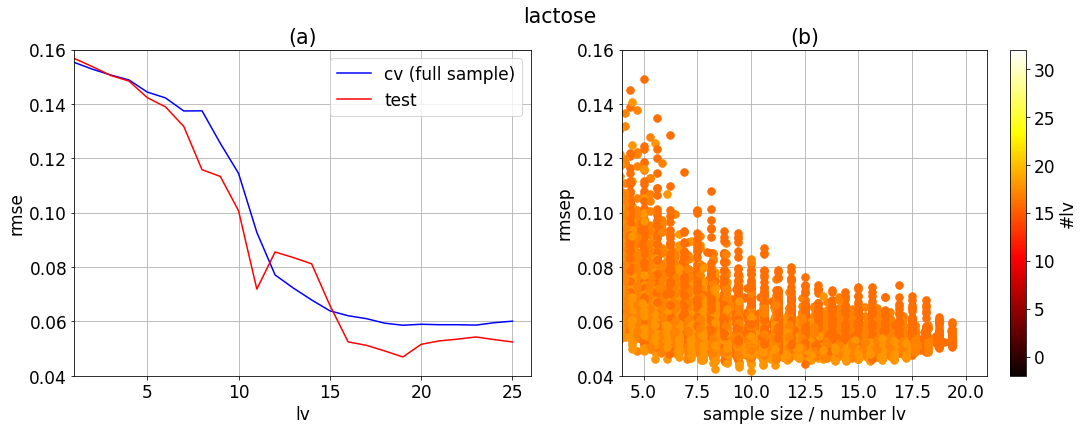
\includegraphics[width=0.8\textwidth]{manuscript/figures/d01_milk_general_framework.png}
\centering
\caption{Evolution of the error (RMSE) in predicting the lactose content in milk from NIR spectra as a function of (a) the number of latent variables $d$; and (b) the ratio of calibration samples over model complexity $(n/d)$ for $d$ values of 16 to 18.}
\label{fig_d01_milk_general_framework}
\end{figure}

\begin{figure}[b]
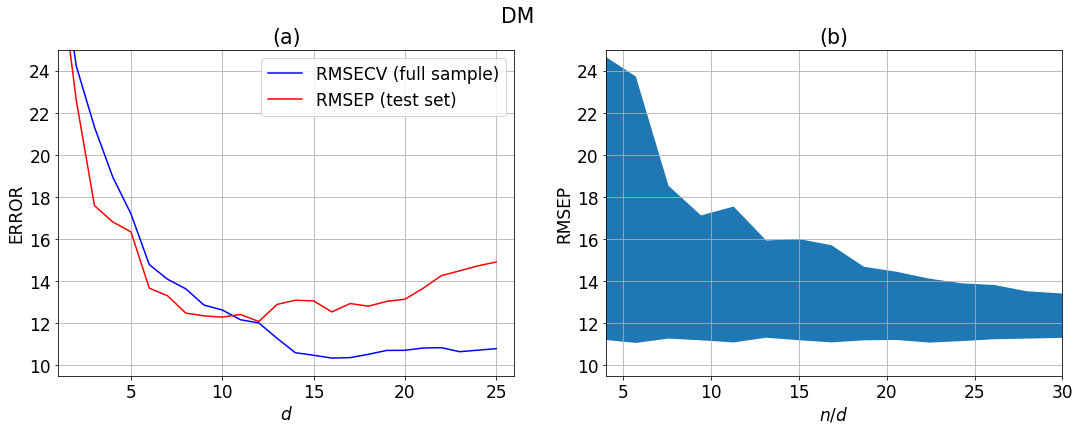
\includegraphics[width=0.8\textwidth]{manuscript/figures/d02_manure_general_framework.png}
\centering
\caption{Evolution of the error (RMSE) in predicting the dry matter content in manure from NIR spectra as a function of (a) the number of latent variables $d$; and (b) the ratio of calibration samples over model complexity $(n/d)$ for $d$ values of 11 to 14.}
\label{fig_d02_manure_general_framework}
\end{figure}

\subsection*{Bilinear modelling as a specific framework}\label{results:specframework}

\emph{What is the effect of input dimensionality, sample size and selection method on the equivalence between $\mathbf{S}_N$ and $\mathbf{S}_n$?} 

As the number of combinations of selection method, sample size and input dimensionality $a$ that has been evaluated is very large, the discussion on the degree of equivalence between $\mathbf{S}_N$ and $\mathbf{S}_n$ is limited to few discrete values of the input dimensionality $a$. The impact of the entire range of $a$ on the model performance is presented in the next section. Figure \ref{fig_specific_framework_detereigevect} shows the comparison of the eigenvectors of $\mathbf{S}_N$ and $\mathbf{S}_n$ for both case studies when the sample selection was made for $a=15$, 20 and 25 with each method. These determinant curves indicated how much equivalence there was between the first $a$ eigenvectors of the matrices as a function of the sample size. These curves demonstrated that, indeed, a small sample size could provide equivalence for a small number of eigenvectors. When more ED directions are accounted for, the equivalence of the eigenvectors requires a larger sample size. 

Across the different methods, the behavior of the determinant at a fixed $a$ was noticeably related to the sample size, yet differently for the different selection methods. Excluding DUP, all the other methods in both case studies showed similar results for $a=15$ and 20. Determinants above 0.8 were achieved with sample sizes below 30\% of $N$. When setting $a=25$ large differences were observed for the selected calibration sets across the different methods and sample sizes. In both case studies, CL and D-OPT selection showed a jump in the determinant around the same sample sizes. In the manure case, KS related to CL and D-OPT in this behavior, while it was PUCH in the milk case. As expected, due to the nature of selection with DUP creating two equivalent subsets, the determinant presents a decline after crossing 50\% of the samples for selection. However, this decline was obtained for $a=20, 25$ and not for $a=15$ indicating the effect of the input dimensionality. RAND selection did not achieve a clear stabilization of the determinant compared to that of the other selection methods. For KS, PUCH, CL and D-OPT, the stabilization of the determinant for $a=25$ in the milk case occurred at $n=200$, as indicated by the discussed ratio $n/d>12$. In the manure case with the same methods, the stabilization could be claimed for $a=20$ at $n=140$ as determined previously by the same ratio. 

The comparison of the resulting individual eigenvalues is presented for the selection made with $a = 25$ for the milk case and with $a=20$ for the manure case in Figures \ref{fig_d01_milk_specific_framework_eigenvalsratio} and \ref{fig_d02_manure_specific_framework_eigenvalsratio}. Each curve represents the eigenvalues ratio for a given value of $n$. With the exception of DUP selection, there is a clear convergence towards 1 of these ratios as $n$ increases. This suggests that, ideally, a subset of samples could be selected such that the resulting eigenvalues are uniformly close to the eigenvalues based on the total number of samples. For small sample sizes, a high variation in the ratios occurred revealing that even when selecting the samples with $a=25$ in the milk case and $a=20$ in the manure case, not all ED directions are equally represented in the subsets. Most interestingly, high peaks and valleys could be observed at the same ED directions indistinctly of the selection method. As $n$ increases, the curves become flatter indicating an equitable representation of the individual ED directions. 

In this comparison, the 50\% effect of DUP selection was detected as the curves for the ratio of the eigenvalues was divided into 2 groups determined by 50\% of the samples. For $n$ larger than 50\% in DUP, the variability starts being underestimated as the curves drop below 1. In both case studies, KS, D-OPT and PUCH selection showed that there is generally no underestimation of variability as the eigenvalues ratio stayed above 1 with very few exceptions. On the other hand, no systematic behavior in the variability of the eigenvalues could be observed for RAND selection. 

As CL is a more robust method compared to the other methods in terms of control over possible outliers, the eigenvalues ratio is overall more stable and closer to 1 in comparison with the other methods. In the milk case, for very small sample sizes, some ED directions resulted in ratios between 0.5 and 1. D-OPT showed more linearity for the eigenvalues ratio as a function of the sample size compared to the other methods in both case studies. 

\begin{table*}[t]
\centering
\begin{tabular}{|cc|cc|} 
\hline
\multicolumn{2}{|c|}{Milk (lactose)} & \multicolumn{2}{|c|}{Manure (DM)}\\
\hline
PC	& correlation	&  PC & correlation	\\
\hline
  1 & -0.1337 & 1 & -0.3132 \\
  2 & -0.1839 & 2 & -0.6231 \\
  3 & -0.0239 & 3 & -0.1587 \\
  4 &  0.2380 & 4 &  0.2220 \\
  5 &  0.0496 & 5 &  0.4036 \\
 16 &  0.0060 & 6 &  0.0299 \\
 17 &  0.0266 & 7 & -0.3102 \\
 18 &  0.4208 & 8 & 0.0521 \\
 19 &  0.1202 & 9 & 0.1543 \\
 20 &  0.0759 & 10& 0.0259 \\
 21 &  0.3819 &  & \\
 \hline
\end{tabular}
\caption{Pearson correlations between PC's and chemical component based on the selection set}
\label{tab_correlations}
\end{table*}

The possible risk of the non-uniform spanning of variability across the different dimensions was supported by the correlations between PC dimensions and the chemical constituent. Table \ref{tab_correlations} shows the Pearson correlations for both case studies. In the case of the milk data set, PC's 18 and 21 showed higher correlations with lactose than PC's 1 and 2. In the manure case, dry matter content had a higher correlation with PC 5 than PC 1, but the first 10 PC's still accounted for the highest correlations. The impact of diminishing or underestimating the variability at certain dimensions should thus be placed in perspective of the PLSR model performance in the next section. With respect to the equivalence between $\mathbf{S}_N$ and $\mathbf{S}_n$, the degree of equivalence depended on the rank value of $a$ and a more uniform span of variability according to the eigenvalues could be obtained in both case studies for sample sizes corresponding to $n/d>12$.  




\begin{figure*}[t]
    \centering
    \subfigure[Milk]{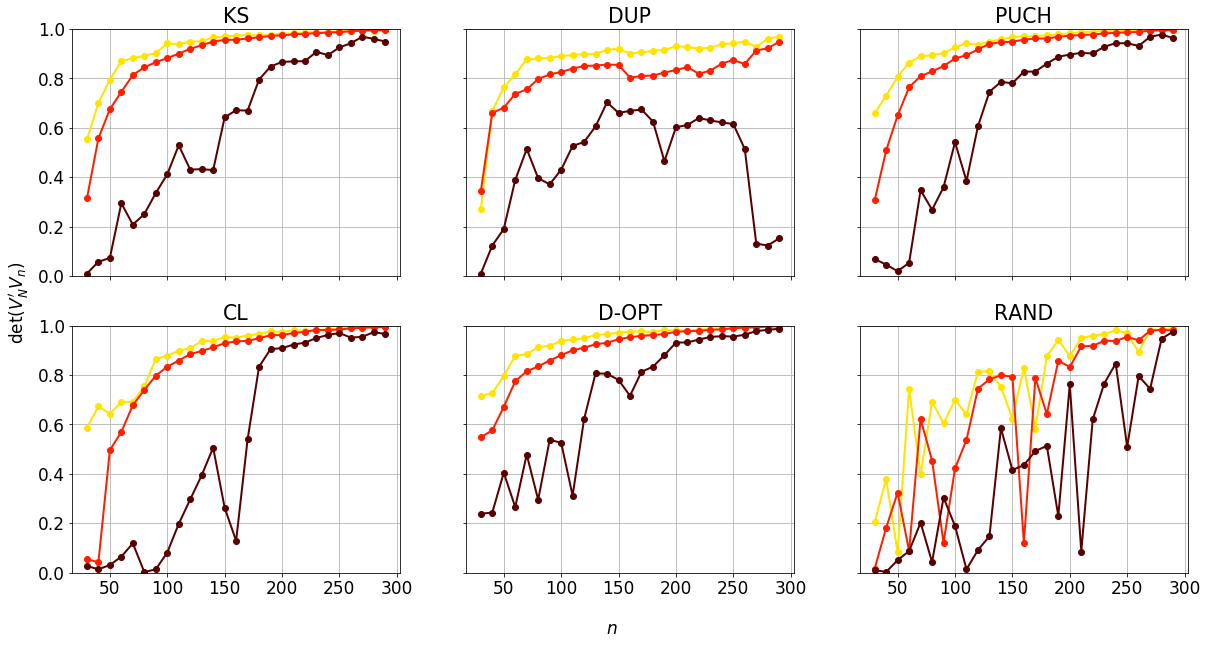
\includegraphics[width=0.6\textwidth]{manuscript/figures/d01_milk_specific_framework_detereigevect.png}} 
    \subfigure[Manure]{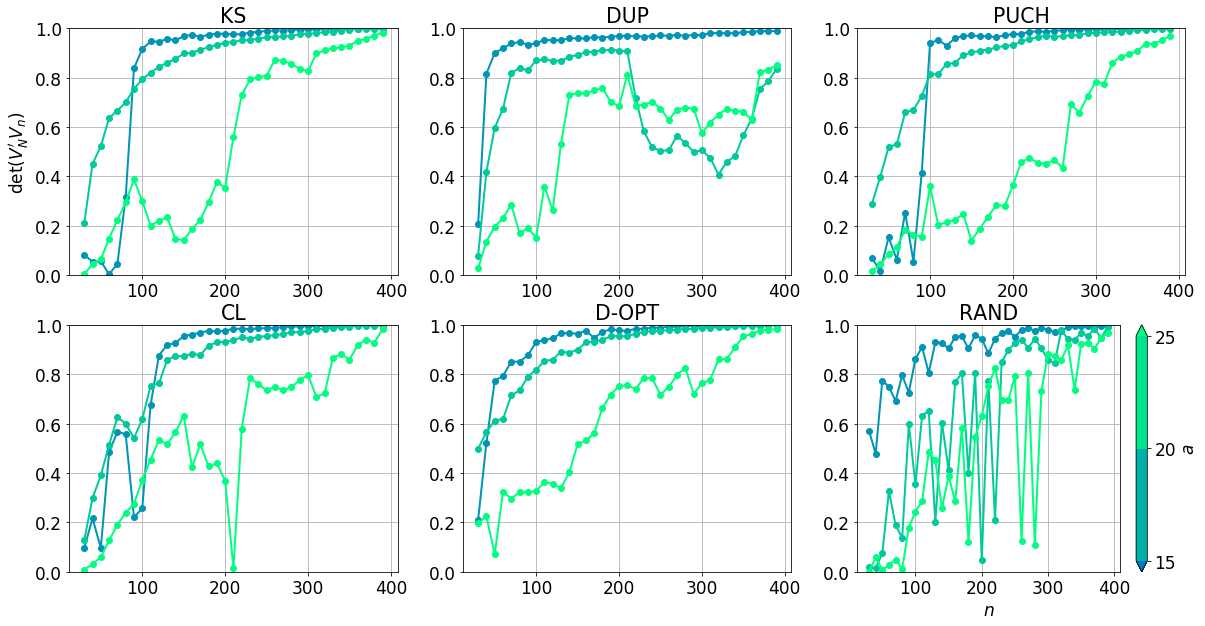
\includegraphics[width=0.6\textwidth]{manuscript/figures/d02_manure_specific_framework_detereigevect.png}}
    \caption{Comparison of eigenvectors when selecting samples with every method and input dimensionality $a=15$ (yellow), $a=20$ (red) and $a=25$ (black).}
    \label{fig_specific_framework_detereigevect}
\end{figure*}

\begin{figure}[b]
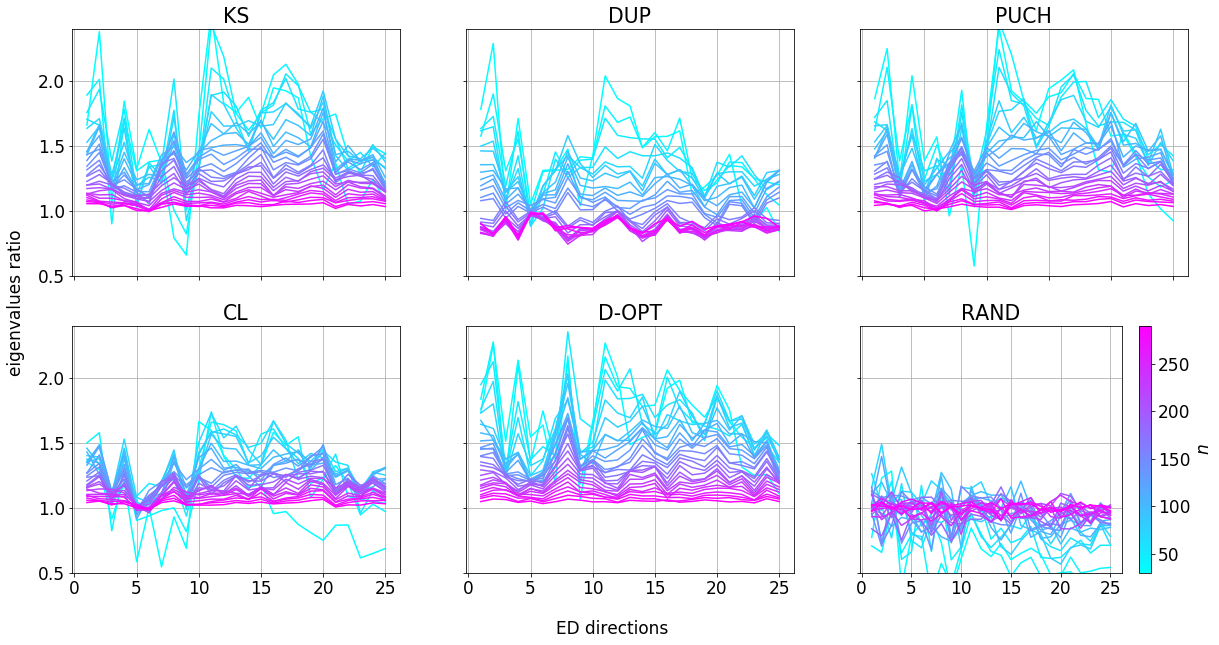
\includegraphics[width=0.8\textwidth]{manuscript/figures/d01_milk_specific_framework_eigenvalsratio.png}
\centering
\caption{Comparison of eigenvalues for the milk case study when selecting samples with every method and input dimensionality $a=25$.}
\label{fig_d01_milk_specific_framework_eigenvalsratio}
\end{figure}

\begin{figure}[b]
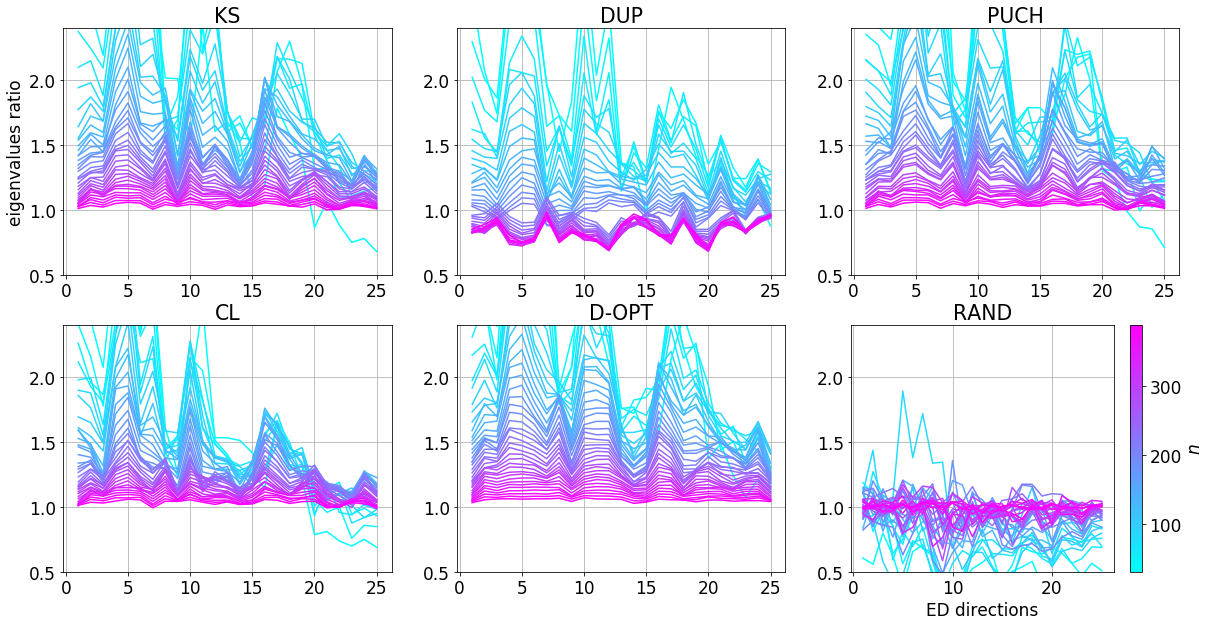
\includegraphics[width=0.8\textwidth]{manuscript/figures/d02_manure_specific_framework_eigenvalsratio.png}
\centering
\caption{Comparison of eigenvalues for the manure case study when selecting samples with every method and input dimensionality $a=25$.}
\label{fig_d02_manure_specific_framework_eigenvalsratio}
\end{figure}

\subsection*{Model performance}\label{results:modperformance}


\emph{What are the most optimal conditions of the three factors for satisfactory PLSR models?}

The simultaneous effect of the three selection factors on the performance of PLSR models was analyzed by comparing the RMSEP curves for each case study. The grid in Figures \ref{fig_d01_milk_model_performance} and \ref{fig_d02_manure_model_performance} shows the PLSR model performance for the milk and the manure case study, respectively. The selection methods are accommodated row-wise, punctual sample sizes are positioned column-wise and the color of the curves represents the input dimensionality. 


\begin{figure}[b]
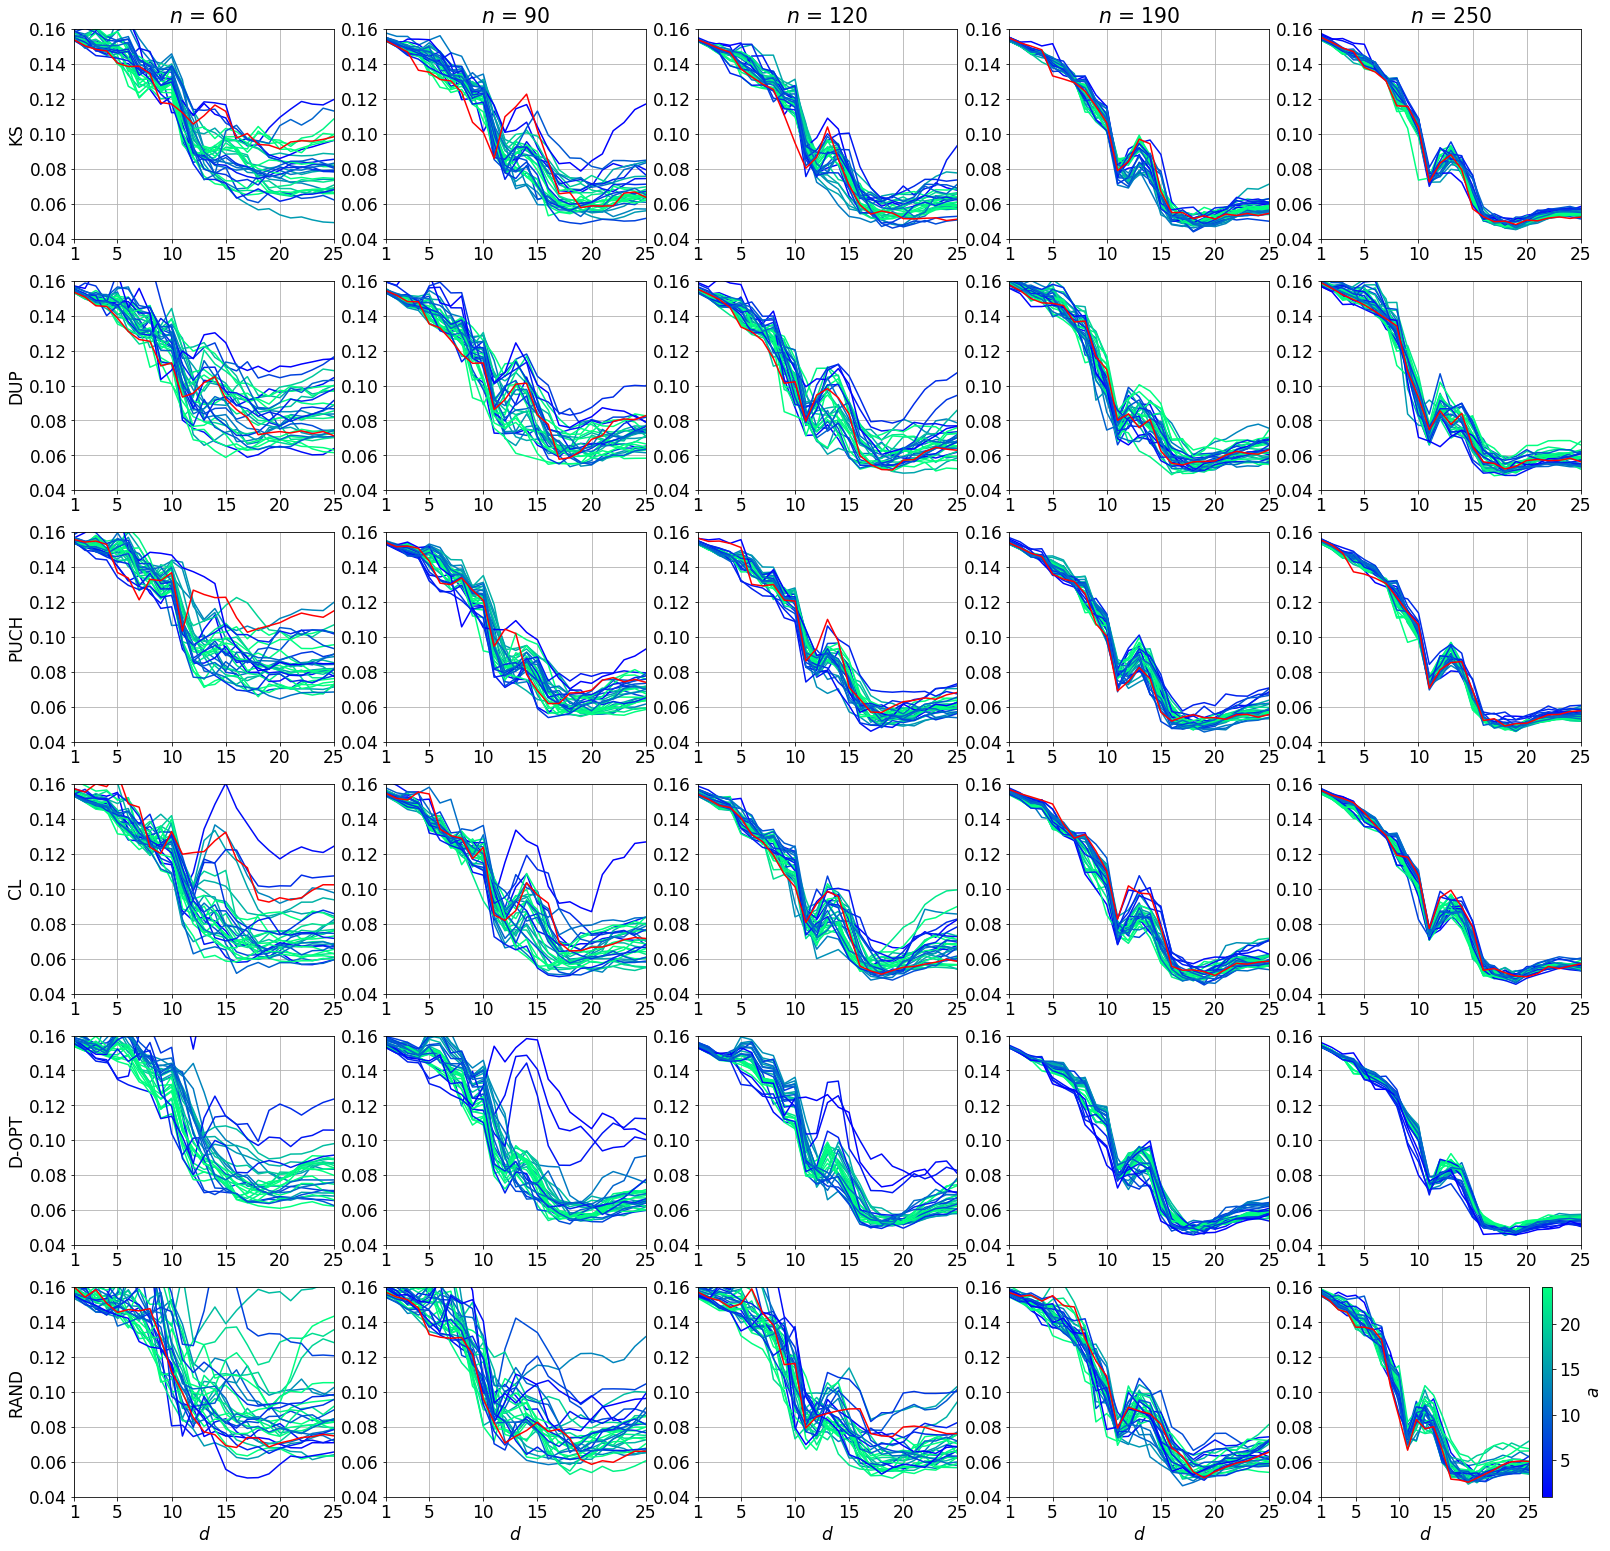
\includegraphics[width=0.8\textwidth]{manuscript/figures/d01_milk_model_performance.png}
\centering
\caption{Model performance to predict lactose content according to selection method, input dimensionality and sample size. The red line represents input dimensionality $a=p$.}
\label{fig_d01_milk_model_performance}
\end{figure}

In both case studies, RAND selection resulted in larger variability in the model performance as the sample size decreased. For sample sizes as large as $260/16 > 16$ in the lactose prediction and $180/11 > 16$ in the prediction of dry matter content, RAND selection rendered calibration sets that were closely optimal to the sets delivered by any other selection method. 

In the prediction of lactose, the model performance for the selected sets of size $n=60$ was highly uncertain and no clear relation was found between a satisfactory performance and the selection method or the input dimensionality. Nonetheless, for such a small $n$, the selected calibration sets by D-OPT with $a \ge 15$ consistently produced models with better performance than the other methods. Similar results were obtained with D-OPT for other small sample sizes ($n=90$ and $n=120$). This differentiation of the effect of the input dimensionality was not equally clear for small sample sizes with the other methods. Moreover, when selecting samples based on the original $\mathbf{X}$ matrix (i.e. $a=p$), there was no satisfactory result for the small sample sizes compared to values of $a$ between 15 and 25. When taking 200 samples, according to 200/16>12, the performance of the models with the different methods and input dimensionality stabilized and no important or systematic difference was observed, especially for RMSEP values at $d=16, 17$ and 18.

The model performances obtained for the manure case suggest similar conclusions on the effect of the factors as in the milk case study. In particular, for small sample sizes such as $n=60$ and $n=90$, D-OPT and PUCH selection showed a more stable performance around $d = 11$ when selecting samples with $a \ge 20$ than the performance stability of the other methods. Once the threshold $n/d>12$ was reached, which happened at 140 samples taking $d=11$, KS, PUCH and D-OPT with $a$ between 20 and 25 rendered calibration sets with satisfactory performance, especially around the optimal complexity. 



\begin{figure}[b]
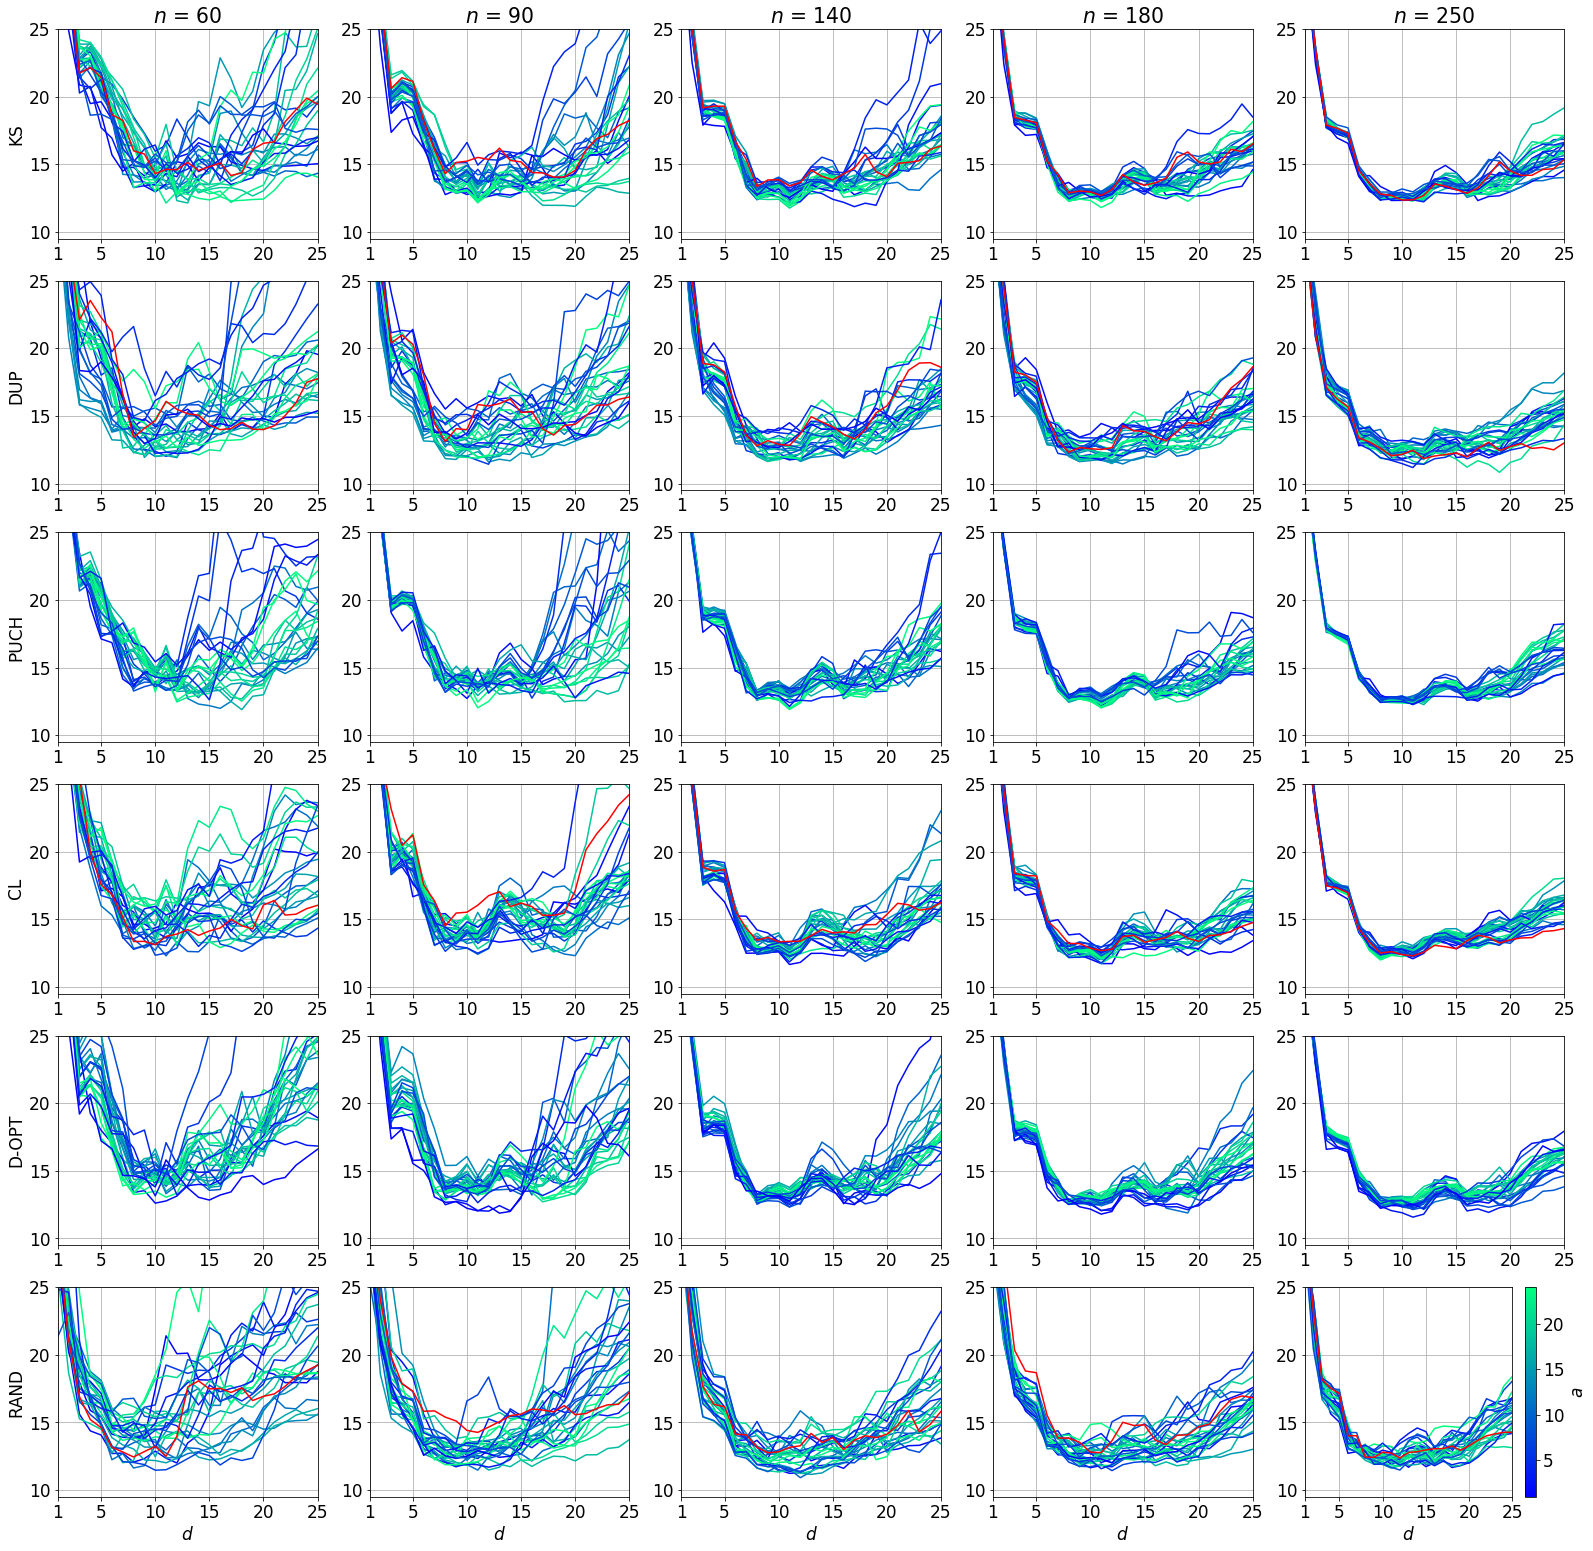
\includegraphics[width=0.8\textwidth]{manuscript/figures/d02_manure_model_performance.png}
\centering
\caption{Model performance to predict dry matter content according to selection method, input dimensionality and sample size. The red line represents input dimensionality $a=p$.}
\label{fig_d02_manure_model_performance}
\end{figure}

% -----------------------------------------------------
% ------------------- discussion  ------------
% -----------------------------------------------------



\section*{Discussion}\label{discussion}

When positioning the PLSR algorithm in the general framework of statistical learning theory, it was found that the sample size needed to establish multivariate calibration models is determined by the $VC$ dimension (i.e. model complexity). This means that a different sample size $n$ will be required for an easy-to-predict dominant chemical constituent than for a minor constituent that is harder to predict. The same idea was commented by Schoot about the sample size for calibration models of different products \cite{Schoot2020}, although no further analysis was provided to explain it. This insight was revealed by the analysis of the ratio $n/d$ and the optimal sample sizes obtained in each case study. The level of easiness to predict is what the $VC$ dimension or model complexity represents. It was confirmed that a ratio $n/d>20$ accounts for a sample size that is rather large for a satisfactory calibration model. Based on the results of the present study, for which a hard-to-predict constituent (lactose in milk) and an easier constituent (dry matter in manure) were analyzed, evidence was obtained that a satisfactory calibration model can be built with $n/d>12$. While unsupervised sample selection is performed at a stage when no data on the target variable $y$ is available yet, it may be possible to estimate $d$ based on the literature and expert knowledge on the problem at hand.

In Au \cite{Au2020}, a threshold for the optimal sample size was found in absolute numbers. For the optimal complexity of 7 to 10 latent variables reported in that study, the stated threshold for the sample size corresponded to a ratio $n/d > 20$. Given that the sample size steps were taken larger, those results still confirm the theory based on the $n/d$ given by Vapnik \cite{Vapnik2000}. Complementary, in the work by Shoot  \cite{Schoot2020}, an absolute threshold of 100 samples was detected to be optimal for calibration models involving some food products. The optimal complexity of the models in the mentioned study was chosen as the location of the minimum RMSECV, which can correspond to RMSECV curves of long tails as it was the case of the milk data for the prediction of lactose content. It is of question whether the sample size threshold of 100 samples corresponded to calibration models that needed about 8 to 10 latent variables as optimal complexity.  

The leading feature to address the current problem is that of spanning as much as possible the variability contained in the original set so that a representative subset of samples is obtained. In the context of chemometrics, this feature had not been concretely translated into a mathematical criterion, which at the same time is to be defined based on the model architecture that best describes the relationship between $\mathbf{X}$ and $y$. The specific framework analysis showed the role that the matrix $\mathbf{S}$ plays in the PLSR model, making it the mathematical element that can be controlled in an unsupervised setting. Therefore, finding a subset of $n$ samples that renders $\mathbf{S}_n$ equivalent to $\mathbf{S}_N$ has been proposed here as a way to define the representativity of the selected samples. 

The results obtained for the comparison of eigenvectors and eigenvalues showed that there is convergence in the equivalence between $\mathbf{S}_n$ and $\mathbf{S}_N$. Naturally, this equivalence depends on the input dimensionality $a$. For the purpose of PLSR model building, the value of $a$ needs to be larger than $d$ and it can be increased up to a value for which equivalence is supported by the fixed sample size based on $n/d>12$. In this way, as many PC dimensions of small variability as possible will be represented by the selected calibration set. From the model performance results obtained when selecting the samples based on a low input dimensionality (i.e. low number of PC's), it became clear that this may greatly compromise the performance of the model after gathering reference analyses. This insight was supported by the model performance achieved with high values of $a$ for KS, CL, PUCH and D-OPT and the high correlations between PC dimensions of low variability and $y$ in the milk case study. While different researchers have reported to reduce the dimensionality for unsupervised sample selection, no general analysis of the effect of this dimensionality reduction was found \cite{Naes1990, Brandmaier2012, Nawar2018, Au2020}. On the other hand, selecting the samples with the original dimensionality of $\mathbf{X}$ was not particularly advantageous over reducing it to $a<<p$. This is relevant for D-OPT which does not support the original matrix $\mathbf{X}$ when its rank is deficient and for PUCH which has been proposed to work with the Mahalanobis distance \cite{Puchwein1988}.

In our study, the effect of the selection method was largely diminished once the sample size and the dimensionality $a$ had been set. Nonetheless, each of the selection methods operates under their own criterion to span the variability. DUP is the least suitable method for unsupervised sample selection as it has been designed to separate the set into two equal subsets containing 50\% of the samples. It functions by finding two replicate submatrices in the matrix $\mathbf{X}$, which might not be the ideal separation according to the threshold $n/d>12$ for the optimal sample size as confirmed by the presented results. However, this method remains suitable to split a data set into calibration and validation during model building\cite{Aernouts2011}. D-OPT selection, on the other hand, proved to consistently deliver an optimal selection for values of $a \ge 15$, considering that less than 10 PC's accounted for more than 95\% of the variability of $\mathbf{X}$ in both case studies. This method, however, is prone to select extreme samples which would render higher eigenvalues with a subset of samples compared to the magnitude achieved with total sample. This fact represents a possible challenge in the presence of bad outliers or an advantage for good leverage points. CL demonstrates to be the most robust strategy for sample selection, although it represents a risk when the sample size $n$ does not correspond to $n$ well-defined groups existing in the original set. This latter insight was hypothesized based on the drop of the determinant rendered by CL in both case studies. CL, KS and PUCH delivered representative calibration sets, but their effect on the model performance did not prove to be better than D-OPT selection. Therefore, a suitable selection criterion would be one that, provided a rank $a$, delivers a set for which $\mathbf{S}_n$ and $\mathbf{S}_N$ are equivalent in terms of their eigenvectors and eigenvalues, subject to a ratio of the eigenvalues above 1 and as uniform as possible across the ED directions.

Regarding the polynomial degree of the input variables, when including only the first order terms, D-OPT unavoidably selects the outer layer of the data variability inwards. The inclusion of higher-order terms is justified under the assumption of nonlinear effects of the input variables on the response variable. As this assumption was not made in the current study and strong nonlinear effects would suggest another model architecture, no higher-order effects were included when using D-OPT sample selection.

Many researchers apply specific data preprocessing techniques to remove certain sources of uninformative variation from the signals. Possible advantages of preprocessing the spectral data prior to unsupervised sample selection have been reported \cite{Liu2019}.
However, initial experiments in the current case studies suggested that assuming advanced preprocessing such as scatter correction resulted in sets rendering calibration models with poor performance. This suggests that strong assumptions related to the required preprocessing prior to obtaining reference analyses are not recommended.

% -----------------------------------------------------
% ------------------- a scheme  ------------
% -----------------------------------------------------

\section*{A guideline for selecting the most informative calibration samples}\label{scheme}

The higher-mentioned conclusions from the exhaustive comparison of the factors involved in unsupervised sample selection can be summarized in a guideline for the establishment of multivariate calibration models, as visualized in Figure \ref{fig_scheme}. After defining a suitable value for the PLSR model complexity $d$ based on expert knowledge and literature, the optimal sample size $n$ can be calculated as 12$d+1$. Once $n$ has been calculated, a value for the input dimensionality $a$ can be found by evaluating at what value of $a>d$ there is convergence in equivalence between $\mathbf{S}_N$ and $\mathbf{S}_n$. This ensures that the dimensions included in the selection account for PC's of small variability that can be beneficial for the PLSR model if a hard-to-predict constituent is involved. The samples can be selected with KS, PUCH, CL or D-OPT, evaluating which method delivers the best equivalence of the covariance matrices based on their eigendecompositions. It is recommended to analyze the presence of potential outliers, in particular when using D-OPT selection. In the presence of outliers, the dimensionality reduction prior to the sample selection can be performed with robust PCA \cite{Hubert2005}.


\begin{figure}[b]
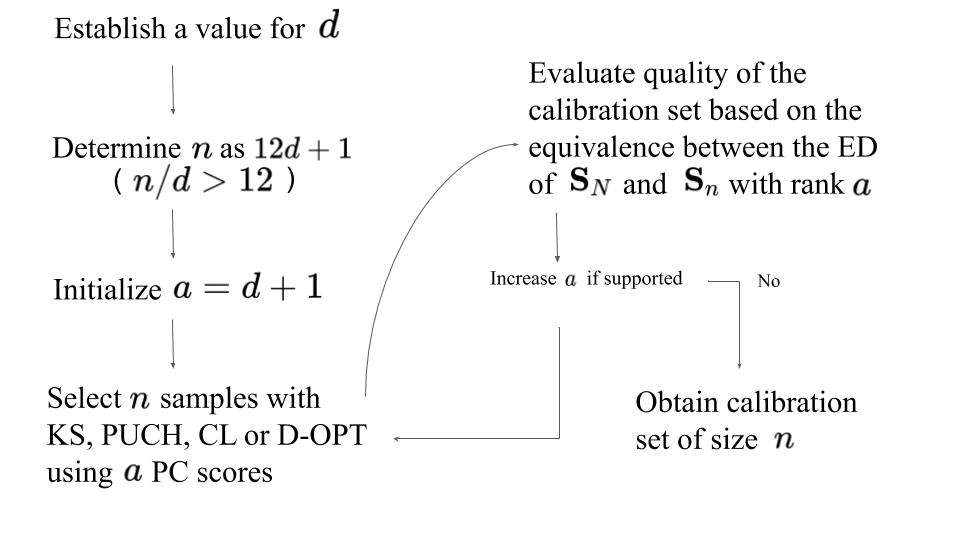
\includegraphics[width=0.6\textwidth]{manuscript/figures/scheme.png}
\centering
\caption{Proposed guideline for unsupervised sample selection in multivariate calibration}
\label{fig_scheme}
\end{figure}

% -----------------------------------------------------
% ------------------- conclusions  ------------
% -----------------------------------------------------

\section*{Conclusions}\label{conclusions}

The positioning of PLSR models in the general framework of statistical learning theory allowed to establish an objective threshold for the optimal sample size to build this type of calibration models, namely $n/d>12$. It was demonstrated that the input dimensionality $a$ plays an important role in the challenge of unsupervised sample selection and that PC dimensions of low variability may still be important to select the most informative samples depending on the dominance of the target chemical constituent. The methods that have been a standard for sample selection in multivariate calibration proved to be equally useful for this challenge after controlling the sample size and the input dimensionality. Random selection was found to require larger sample sizes. 

The proposed scheme was developed in the context of PLSR models. However, most model architectures, including nonlinear models such as neural networks or support vector machines relate to a $VC$ dimension which can be theoretically determined or practically estimated \cite{Vapnik2019, Vapnik1994}. This is also not restricted only to regression models, the same ideas apply for classification models. This means that optimal sample sizes can be calculated based on the ratio $n/d$ if an estimate for the model complexity $d$ can be found for the problem at hand. 

The criterion based on the equivalence between $\mathbf{S}_N$ and $\mathbf{S}_n$ is specific for bilinear models such as PLSR, PLS discriminant analysis, linear regression, among others. Further research is recommended to refine this criterion of equivalence and to propose a sample selection algorithm aimed at optimizing this equivalence. This concept could be extended to other model architectures by identifying the mathematical components that could be controlled in unsupervised sample selection \cite{Li2020}. 


% -----------------------------------------------------
% ------------------- data availability  ------------
% -----------------------------------------------------

\section{Data availability}

All the methodology and data that was used in the present work is available for public share. 

% -----------------------------------------------------
% ------------------- acknowledgements  ------------
% -----------------------------------------------------

\begin{acknowledgement}

Valeria Fonseca Diaz is funded as aspirant to doctoral fellow of
the Research Foundation-Flanders (FWO Brussels, Belgium).
The authors thank Dr. Raffaele Vitale and professor Peter Goos (KU Leuven, Belgium) for their suggestions on the conducted analysis given their expertise in Chemometrics and Experimental Design. 
\end{acknowledgement}

% -----------------------------------------------------
% ------------------- bibliography  ------------
% -----------------------------------------------------



\bibliography{biblio}


\end{document}

